% Options for packages loaded elsewhere
\PassOptionsToPackage{unicode}{hyperref}
\PassOptionsToPackage{hyphens}{url}
%
\documentclass[
  ignorenonframetext,
  usenames,
  dvipsnames]{beamer}
\usepackage{pgfpages}
\setbeamertemplate{caption}[numbered]
\setbeamertemplate{caption label separator}{: }
\setbeamercolor{caption name}{fg=normal text.fg}
\beamertemplatenavigationsymbolsempty
% Prevent slide breaks in the middle of a paragraph
\widowpenalties 1 10000
\raggedbottom
\setbeamertemplate{part page}{
  \centering
  \begin{beamercolorbox}[sep=16pt,center]{part title}
    \usebeamerfont{part title}\insertpart\par
  \end{beamercolorbox}
}
\setbeamertemplate{section page}{
  \centering
  \begin{beamercolorbox}[sep=12pt,center]{part title}
    \usebeamerfont{section title}\insertsection\par
  \end{beamercolorbox}
}
\setbeamertemplate{subsection page}{
  \centering
  \begin{beamercolorbox}[sep=8pt,center]{part title}
    \usebeamerfont{subsection title}\insertsubsection\par
  \end{beamercolorbox}
}
\AtBeginPart{
  \frame{\partpage}
}
\AtBeginSection{
  \ifbibliography
  \else
    \frame{\sectionpage}
  \fi
}
\AtBeginSubsection{
  \frame{\subsectionpage}
}
\usepackage{amsmath,amssymb}
\usepackage{lmodern}
\usepackage{iftex}
\ifPDFTeX
  \usepackage[T1]{fontenc}
  \usepackage[utf8]{inputenc}
  \usepackage{textcomp} % provide euro and other symbols
\else % if luatex or xetex
  \usepackage{unicode-math}
  \defaultfontfeatures{Scale=MatchLowercase}
  \defaultfontfeatures[\rmfamily]{Ligatures=TeX,Scale=1}
\fi
\usetheme[]{CambridgeUS}
\usecolortheme{crane}
\usefonttheme{structurebold}
% Use upquote if available, for straight quotes in verbatim environments
\IfFileExists{upquote.sty}{\usepackage{upquote}}{}
\IfFileExists{microtype.sty}{% use microtype if available
  \usepackage[]{microtype}
  \UseMicrotypeSet[protrusion]{basicmath} % disable protrusion for tt fonts
}{}
\makeatletter
\@ifundefined{KOMAClassName}{% if non-KOMA class
  \IfFileExists{parskip.sty}{%
    \usepackage{parskip}
  }{% else
    \setlength{\parindent}{0pt}
    \setlength{\parskip}{6pt plus 2pt minus 1pt}}
}{% if KOMA class
  \KOMAoptions{parskip=half}}
\makeatother
\usepackage{xcolor}
\newif\ifbibliography
\usepackage{color}
\usepackage{fancyvrb}
\newcommand{\VerbBar}{|}
\newcommand{\VERB}{\Verb[commandchars=\\\{\}]}
\DefineVerbatimEnvironment{Highlighting}{Verbatim}{commandchars=\\\{\}}
% Add ',fontsize=\small' for more characters per line
\usepackage{framed}
\definecolor{shadecolor}{RGB}{248,248,248}
\newenvironment{Shaded}{\begin{snugshade}}{\end{snugshade}}
\newcommand{\AlertTok}[1]{\textcolor[rgb]{0.94,0.16,0.16}{#1}}
\newcommand{\AnnotationTok}[1]{\textcolor[rgb]{0.56,0.35,0.01}{\textbf{\textit{#1}}}}
\newcommand{\AttributeTok}[1]{\textcolor[rgb]{0.77,0.63,0.00}{#1}}
\newcommand{\BaseNTok}[1]{\textcolor[rgb]{0.00,0.00,0.81}{#1}}
\newcommand{\BuiltInTok}[1]{#1}
\newcommand{\CharTok}[1]{\textcolor[rgb]{0.31,0.60,0.02}{#1}}
\newcommand{\CommentTok}[1]{\textcolor[rgb]{0.56,0.35,0.01}{\textit{#1}}}
\newcommand{\CommentVarTok}[1]{\textcolor[rgb]{0.56,0.35,0.01}{\textbf{\textit{#1}}}}
\newcommand{\ConstantTok}[1]{\textcolor[rgb]{0.00,0.00,0.00}{#1}}
\newcommand{\ControlFlowTok}[1]{\textcolor[rgb]{0.13,0.29,0.53}{\textbf{#1}}}
\newcommand{\DataTypeTok}[1]{\textcolor[rgb]{0.13,0.29,0.53}{#1}}
\newcommand{\DecValTok}[1]{\textcolor[rgb]{0.00,0.00,0.81}{#1}}
\newcommand{\DocumentationTok}[1]{\textcolor[rgb]{0.56,0.35,0.01}{\textbf{\textit{#1}}}}
\newcommand{\ErrorTok}[1]{\textcolor[rgb]{0.64,0.00,0.00}{\textbf{#1}}}
\newcommand{\ExtensionTok}[1]{#1}
\newcommand{\FloatTok}[1]{\textcolor[rgb]{0.00,0.00,0.81}{#1}}
\newcommand{\FunctionTok}[1]{\textcolor[rgb]{0.00,0.00,0.00}{#1}}
\newcommand{\ImportTok}[1]{#1}
\newcommand{\InformationTok}[1]{\textcolor[rgb]{0.56,0.35,0.01}{\textbf{\textit{#1}}}}
\newcommand{\KeywordTok}[1]{\textcolor[rgb]{0.13,0.29,0.53}{\textbf{#1}}}
\newcommand{\NormalTok}[1]{#1}
\newcommand{\OperatorTok}[1]{\textcolor[rgb]{0.81,0.36,0.00}{\textbf{#1}}}
\newcommand{\OtherTok}[1]{\textcolor[rgb]{0.56,0.35,0.01}{#1}}
\newcommand{\PreprocessorTok}[1]{\textcolor[rgb]{0.56,0.35,0.01}{\textit{#1}}}
\newcommand{\RegionMarkerTok}[1]{#1}
\newcommand{\SpecialCharTok}[1]{\textcolor[rgb]{0.00,0.00,0.00}{#1}}
\newcommand{\SpecialStringTok}[1]{\textcolor[rgb]{0.31,0.60,0.02}{#1}}
\newcommand{\StringTok}[1]{\textcolor[rgb]{0.31,0.60,0.02}{#1}}
\newcommand{\VariableTok}[1]{\textcolor[rgb]{0.00,0.00,0.00}{#1}}
\newcommand{\VerbatimStringTok}[1]{\textcolor[rgb]{0.31,0.60,0.02}{#1}}
\newcommand{\WarningTok}[1]{\textcolor[rgb]{0.56,0.35,0.01}{\textbf{\textit{#1}}}}
\usepackage{graphicx}
\makeatletter
\def\maxwidth{\ifdim\Gin@nat@width>\linewidth\linewidth\else\Gin@nat@width\fi}
\def\maxheight{\ifdim\Gin@nat@height>\textheight\textheight\else\Gin@nat@height\fi}
\makeatother
% Scale images if necessary, so that they will not overflow the page
% margins by default, and it is still possible to overwrite the defaults
% using explicit options in \includegraphics[width, height, ...]{}
\setkeys{Gin}{width=\maxwidth,height=\maxheight,keepaspectratio}
% Set default figure placement to htbp
\makeatletter
\def\fps@figure{htbp}
\makeatother
\usepackage[normalem]{ulem}
\setlength{\emergencystretch}{3em} % prevent overfull lines
\providecommand{\tightlist}{%
  \setlength{\itemsep}{0pt}\setlength{\parskip}{0pt}}
\setcounter{secnumdepth}{-\maxdimen} % remove section numbering
\newlength{\cslhangindent}
\setlength{\cslhangindent}{1.5em}
\newlength{\csllabelwidth}
\setlength{\csllabelwidth}{3em}
\newlength{\cslentryspacingunit} % times entry-spacing
\setlength{\cslentryspacingunit}{\parskip}
\newenvironment{CSLReferences}[2] % #1 hanging-ident, #2 entry spacing
 {% don't indent paragraphs
  \setlength{\parindent}{0pt}
  % turn on hanging indent if param 1 is 1
  \ifodd #1
  \let\oldpar\par
  \def\par{\hangindent=\cslhangindent\oldpar}
  \fi
  % set entry spacing
  \setlength{\parskip}{#2\cslentryspacingunit}
 }%
 {}
\usepackage{calc}
\newcommand{\CSLBlock}[1]{#1\hfill\break}
\newcommand{\CSLLeftMargin}[1]{\parbox[t]{\csllabelwidth}{#1}}
\newcommand{\CSLRightInline}[1]{\parbox[t]{\linewidth - \csllabelwidth}{#1}\break}
\newcommand{\CSLIndent}[1]{\hspace{\cslhangindent}#1}
\newenvironment{cols}[1][]{}{}

\newenvironment{col}[1]{\begin{minipage}{#1}\ignorespaces}{%
\end{minipage}
\ifhmode\unskip\fi
\aftergroup\useignorespacesandallpars}

\def\useignorespacesandallpars#1\ignorespaces\fi{%
#1\fi\ignorespacesandallpars}

\makeatletter
\def\ignorespacesandallpars{%
  \@ifnextchar\par
    {\expandafter\ignorespacesandallpars\@gobble}%
    {}%
}
\makeatother
\setbeamertemplate{footline}
{%
\begin{beamercolorbox}[wd = 0.2\textwidth, ht = 3ex, dp = 1.5ex, leftskip = .5em, rightskip = .5em]{title in head/foot}%
  \usebeamerfont{title in head/foot}%
  Bacri \hfill%
\end{beamercolorbox}%
\vspace*{-4.5ex}
\hspace*{0.2\textwidth}%
\begin{beamercolorbox}[wd = 0.9\textwidth, ht = 3ex, dp = 1.5ex, leftskip = .5em, rightskip = .5em]{title in head/foot}%
  \usebeamerfont{title in head/foot}%
  \insertshorttitle \hfill%
\end{beamercolorbox}%
\vspace*{-4.5ex}
\hspace*{0.9\textwidth}%
\begin{beamercolorbox}[wd = 0.5\textwidth, ht = 3ex, dp = 1.5ex, leftskip = 0.5em, rightskip = .5em]{author in head/foot}%
  \usebeamerfont{author in head/foot}%
  \insertframenumber{} of \inserttotalframenumber \hfill %\insertshortauthor
\end{beamercolorbox}%
}
\setbeamertemplate{navigation symbols}{}


\definecolor{backgroundColour}{rgb}{0.97,0.96,0.97}
\usepackage{bm}
\usepackage{listings}
\lstset {
  language={C++},
  numbers=none,
  frame=none,
  includerangemarker=false,
  basicstyle=\tiny\ttfamily, % basic font setting
  backgroundcolor=\color{backgroundColour},
% https://tex.stackexchange.com/questions/68091/how-do-i-add-syntax-coloring-to-my-c-source-code-in-beamer
  keywordstyle=\color{BlueViolet}\textbf,
  emph={DATA_VECTOR, DATA_INTEGER, PARAMETER, PARAMETER_VECTOR, sum, exp, dnorm, Type, dpois, size,
		Gamma_w2n, Stat_dist, ADREPORT, objective_function, setOnes,
        row, vector, matrix},
  emphstyle=\color{MidnightBlue}\textbf,
  % emph={[2]a, b, x, y, m, n, i, j, sigma, tsigma, nll},
  % emphstyle={[2]\color{Green}},
  commentstyle=\color{Brown}\textit,
  % morecomment=[l][\color{magenta}]{\#}
}
\providecommand{\J}{J\"{o}reskog}
\providecommand{\So}{S\"{o}rbom}
\providecommand{\bcx}{{\bf X}}
\providecommand{\bcy}{{\bf Y}}
\providecommand{\bcz}{{\bf Z}}
\providecommand{\bcu}{{\bf U}}
\providecommand{\bcv}{{\bf V}}
\providecommand{\bcw}{{\bf W}}
\providecommand{\bci}{{\bf I}}
\providecommand{\bch}{{\bf H}}
\providecommand{\bcb}{{\bf B}}
\providecommand{\bcr}{{\bf R}}
\providecommand{\bcm}{{\bf M}}
\providecommand{\bcp}{{\bf P}}
\providecommand{\bcf}{{\bf F}}
\providecommand{\bcg}{{\bf G}}
\providecommand{\bcs}{{\bf S}}
\providecommand{\bct}{{\bf T}}
\providecommand{\bca}{{\bf A}}
\providecommand{\bcd}{{\bf D}}
\providecommand{\bcc}{{\bf C}}
\providecommand{\bce}{{\bf E}}
\providecommand{\ba}{{\bf a}}
\providecommand{\bb}{{\bf b}}
\providecommand{\bc}{{\bf c}}
\providecommand{\bd}{{\bf d}}
\providecommand{\bx}{\mbox{\boldmath x}}
\providecommand{\by}{\mbox{\boldmath y}}
\providecommand{\bz}{{\bf z}}
\providecommand{\bu}{{\bf u}}
\providecommand{\bv}{{\bf v}}
\providecommand{\bh}{{\bf h}}
\providecommand{\bl}{{\bf l}}
\providecommand{\be}{{\bf e}}
\providecommand{\br}{{\bf r}}
\providecommand{\bw}{{\bf w}}
\providecommand{\de}{\stackrel{D}{=}}
\providecommand{\bt}{\bigtriangleup}
\providecommand{\bfequiv}{\mbox{\boldmath $\equiv$}}
\providecommand{\bmu}{\mbox{\boldmath $\mu$}}
\providecommand{\bnu}{\mbox{\boldmath $\nu$}}
\providecommand{\bxi}{\mbox{\boldmath $\xi$}}
\providecommand{\btau}{\mbox{\boldmath $\tau$}}
\providecommand{\bgamma}{\mbox{\boldmath $\Gamma$}}
\providecommand{\bphi}{\mbox{\boldmath $\Phi$}}
\providecommand{\bfphi}{\mbox{\boldmath $\varphi$}}
\providecommand{\bfeta}{\mbox{\boldmath $\eta$}}
\providecommand{\bpi}{\mbox{\boldmath $\Pi$}}
\providecommand{\bequiv}{\mbox{\boldmath $\equiv$}}
\providecommand{\bvarepsilon}{\mbox{\boldmath $\varepsilon$}}
\providecommand{\btriangle}{\mbox{\boldmath $\triangle$}}
\providecommand{\bdelta}{\mbox{\boldmath $\Delta$}}
\providecommand{\beps}{\mbox{\boldmath $\epsilon$}}
\providecommand{\btheta}{\mbox{\boldmath $\theta$}}
\providecommand{\balpha}{\mbox{\boldmath $\alpha$}}
\providecommand{\bfbeta}{\mbox{\boldmath $\beta$}}
\providecommand{\bsphi}{\mbox{\boldmath $\varphi$}}
\providecommand{\bsig}{\mbox{\boldmath $\sigma$}}
\providecommand{\bfpsi}{\mbox{\boldmath $\psi$}}
\providecommand{\bfdelta}{\mbox{\boldmath $\delta$}}
\providecommand{\bsigma}{{\bf \Sigma}}
\providecommand{\bzero}{{\bf 0}}
\providecommand{\bone}{{\bf 1}}
\providecommand{\bpsi}{\mbox{\boldmath $\Psi$}}
\providecommand{\bep}{\mbox{\boldmath $\epsilon$}}
\providecommand{\bomega}{\mbox{\boldmath $\Omega$}}
\providecommand{\bfomega}{\mbox{\boldmath $\omega$}}
\providecommand{\blambda}{\mbox{\boldmath $\Lambda$}}
\providecommand{\bflambda}{\mbox{\boldmath $\lambda$}}
\providecommand{\bfsigma}{\mbox{\boldmath $\sigma$}}
\providecommand{\bfpi}{{\mbox{\boldmath $\pi$}}}
\providecommand{\bupsilon}{\mbox{\boldmath $\upsilon$}}
\providecommand{\obs}{{\rm obs}}
\providecommand{\mis}{{\rm mis}}
\providecommand{\bs}[1]{\mbox{\boldmath $#1$}}
\titlegraphic{
\includegraphics[width = 3cm]{UiB logo rainbow.jpg}}
\usepackage{movie15}
\ifLuaTeX
  \usepackage{selnolig}  % disable illegal ligatures
\fi
\IfFileExists{bookmark.sty}{\usepackage{bookmark}}{\usepackage{hyperref}}
\IfFileExists{xurl.sty}{\usepackage{xurl}}{} % add URL line breaks if available
\urlstyle{same} % disable monospaced font for URLs
\hypersetup{
  pdftitle={Introduction to parallel processing},
  pdfauthor={Timothée BacriUniversity of Bergen},
  hidelinks,
  pdfcreator={LaTeX via pandoc}}

\title{Introduction to parallel processing}
\author{Timothée Bacri\newline University of Bergen}
\date{06 December, 2022}

\begin{document}
\frame{\titlepage}

\hypertarget{how-to-achieve-high-performance}{%
\section{How to achieve high
performance}\label{how-to-achieve-high-performance}}

\begin{frame}[fragile]{Specialization}
\protect\hypertarget{specialization}{}
\small

\begin{block}{Hardware}
\protect\hypertarget{hardware}{}
\begin{itemize}
\tightlist
\item
  Powerful CPU
\item
  Recent CPU
\item
  CPUs with instruction sets AES-NI / AVX / other
\item
  GPUs for image processing
\end{itemize}
\end{block}

\begin{block}{Software}
\protect\hypertarget{software}{}
\begin{itemize}
\tightlist
\item
  \texttt{ADMB}, \texttt{TMB}
\item
  BLAS (Basic Linear Algebra Subroutines) libraries for basic vector and
  matrix operations
\item
  LAPACK (Linear Algebra Package) libraries for solving systems of
  equation, matrix factorization, eigenvalue
\item
  Approximations
\item
  Automatic parallelization by the compiler (e.g.~Haskell)
\end{itemize}
\end{block}

\begin{block}{Both}
\protect\hypertarget{both}{}
\begin{itemize}
\tightlist
\item
  Parallelization
\end{itemize}

\normalsize
\end{block}
\end{frame}

\hypertarget{introduction-to-parallel-processing}{%
\section{Introduction to parallel
processing}\label{introduction-to-parallel-processing}}

\begin{frame}[fragile]{Terminology}
\protect\hypertarget{terminology}{}
\begin{block}{Hardware}
\protect\hypertarget{hardware-1}{}
\begin{itemize}
\tightlist
\item
  \textbf{Processor / CPU}: Electrical circuit that performs basic
  operations on external data.
\item
  \textbf{Core}: Processing unit.
\item
  \textbf{Cluster}: Collection (of machines/cores).
\end{itemize}
\end{block}

\begin{block}{Software}
\protect\hypertarget{software-1}{}
\begin{itemize}
\tightlist
\item
  \textbf{Thread}: Sequence of instructions in a process.
\item
  \textbf{Process}: Running instance of \texttt{R}.
\item
  \textbf{Socket}: Duplicated process, uses duplicated memory.
\item
  \textbf{Fork}: Duplicated process, uses copy-on-write mechanism.
\end{itemize}
\end{block}

\begin{block}{Language update}
\protect\hypertarget{language-update}{}
\sout{Master/slave} main/worker, parent/child, chief/worker\ldots{}
\end{block}
\end{frame}

\begin{frame}{Types}
\protect\hypertarget{types}{}
\begin{block}{Socket}
\protect\hypertarget{socket}{}
\begin{itemize}
\tightlist
\item
  Works on any system and on clusters
\item
  Uses more resources
\item
  Little slower
\end{itemize}
\end{block}

\begin{block}{Forking}
\protect\hypertarget{forking}{}
\begin{itemize}
\tightlist
\item
  Single machine
\item
  Unix-like operating systems e.g.~Linux distributions and macOS
\item
  Uses less resources
\item
  Little faster
\end{itemize}
\end{block}
\end{frame}

\begin{frame}[fragile]{Brief history}
\protect\hypertarget{brief-history}{}
\begin{itemize}
\tightlist
\item
  \texttt{snow} (Simple Network of Workstations) (2003) with
  \texttt{doSNOW}
\item
  \texttt{multicore} (2009) with \texttt{doMC} (uses forking)
\end{itemize}

Wrappers:

\begin{itemize}
\tightlist
\item
  \texttt{parallel} (2011) with \texttt{doParallel}
\item
  \texttt{future} (2015) with \texttt{dofuture}
\end{itemize}

More details at
\url{https://cran.r-project.org/web/views/HighPerformanceComputing.html}
\end{frame}

\begin{frame}{Where to parallelize}
\protect\hypertarget{where-to-parallelize}{}
When all tasks are independent, so-called embarrassingly parallel
problems (or perfectly, delightfully, pleasingly)

\begin{itemize}
\tightlist
\item
  Monte-Carlo simulations
\item
  Numerical integration
\item
  Computer graphics
\item
  Brute-force searches in cryptography
\item
  Search of hyper parameters in machine learning
\item
  Genetic optimization algorithms
\item
  Cross-validation
\item
  Random forests
\end{itemize}

Non-embarrassingly parallel problems are more difficult to parallelize.
\end{frame}

\begin{frame}{Should I parallelize? (1)}
\protect\hypertarget{should-i-parallelize-1}{}
Time required to write the code \& overhead \& resources v.s. speedup.

\begin{block}{Amdahl's law (1967)}
Maximum speedup in latency (inverse of task speed)
\[
S(N, p) = \frac{T}{T_{N \text{ cores}}} = \frac{(1-p)T + pT}{(1-p)T + \frac{pT}{N}} = \frac{1}{1-p+\frac{p}{N}}
\]
\begin{itemize}
  \itemsep 0em
  \item \(S\) = speedup of the task's latency
  \item \(N\) = cores
  \item \(p\) = \% task benefiting from parallelization
  \item \(T\) = time with 1 core
\end{itemize}
\end{block}

\begin{block}{Example}
If 50\% of a problem is sped up (\(p = 0.5\)) by a factor of 10 (\(N = 10\)), then the maximum speedup is \(S(2, 0.5) = 1.82\).
\end{block}
\end{frame}

\begin{frame}{Should I parallelize? (2)}
\protect\hypertarget{should-i-parallelize-2}{}
\begin{block}{Gustafson's law (1988)}
\[
S(N, p) = \frac{T}{T_{N \text{ cores}}} = \frac{(1-p)T + NpT}{(1 - p) T + \frac{NpT}{N}} = 1 + p(N - 1)
\]
\begin{itemize}
  \itemsep 0em
  \item \(S\) = speedup of the task's latency
  \item \(N\) = cores
  \item \(p\) = \% task benefiting from parallelization
  \item \(T\) = time with 1 core before parallelization
\end{itemize}
\end{block}

Assumes that the parallelizable work is multiplied by \(N\) when
parallelized.

\begin{block}{Example}
If 50\% of a problem is sped up (\(p = 0.5\)) by a factor of 10 (\(N = 10\)), then the maximum speedup is \(S(2, 0.5) = 5.5\).
\end{block}
\end{frame}

\begin{frame}{Should I parallelize? (3)}
\protect\hypertarget{should-i-parallelize-3}{}
\begin{block}{Sun-Ni's law (1990), memory-bounded speedup, simplified}
\[
S(N, p) = \frac{T}{T_{N \text{ cores}}} = \frac{(1-p)T + g(N)pT}{(1 - p) T + \frac{g(N)pT}{N}} = \frac{(1-p) + g(N)p}{(1 - p)  + \frac{g(N)p}{N}}
\]
\begin{itemize}
  \itemsep 0em
  \item \(S\) = speedup of the task's latency
  \item \(N\) = cores
  \item \(p\) = \% task benefiting from parallelization
  \item \(T\) = time with 1 core before parallelization
\end{itemize}
\end{block}

Assumes that the parallelizable work is multiplied by \(g(N)\) when
parallelized.
\end{frame}

\begin{frame}{Parallel slowdown}
\protect\hypertarget{parallel-slowdown}{}
Non-embarrassingly parallel tasks require communication between
processes, which slows down the program.

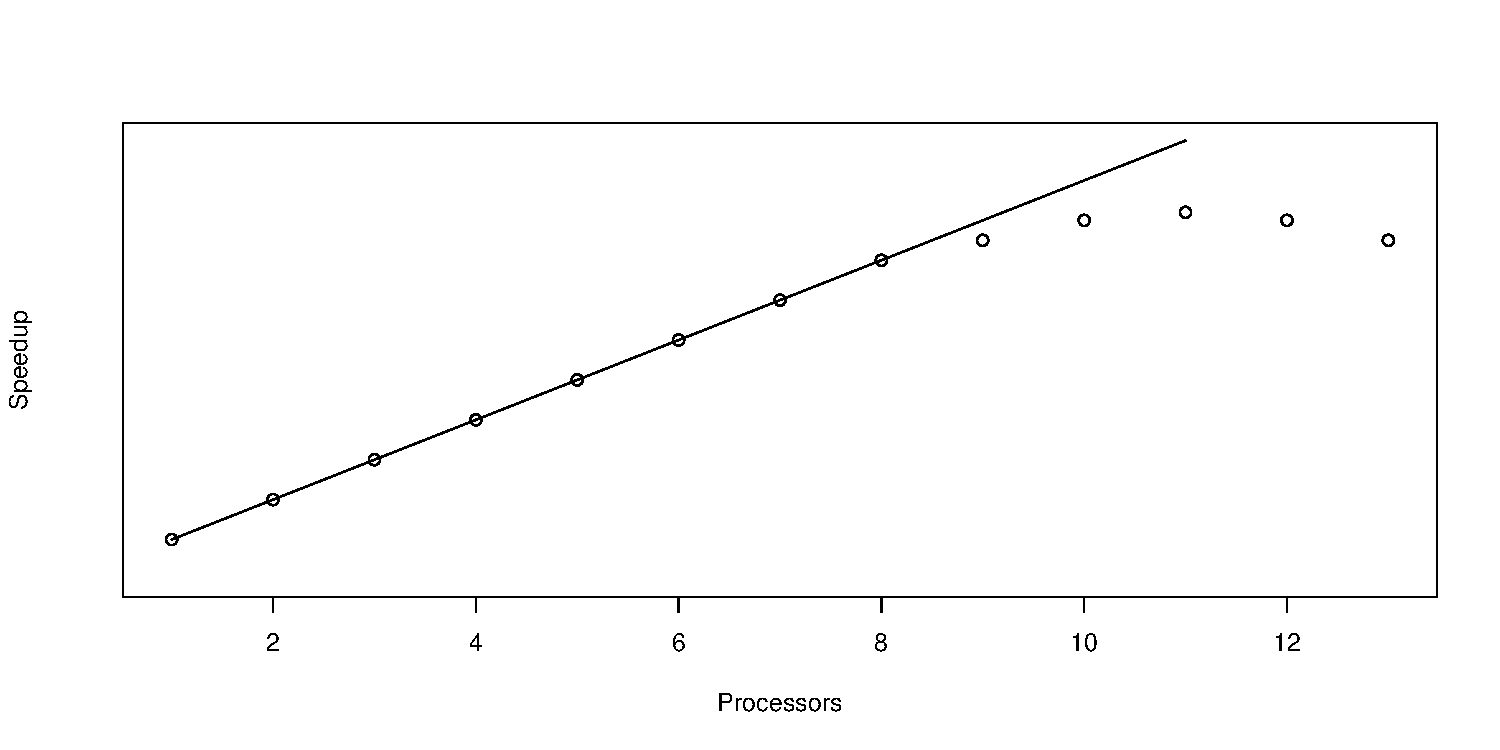
\includegraphics{fast_computing_files/figure-beamer/unnamed-chunk-1-1.pdf}
\end{frame}

\hypertarget{embarassingly-parallel-problem}{%
\section{Embarassingly parallel
problem}\label{embarassingly-parallel-problem}}

\begin{frame}{Big Data}
\protect\hypertarget{big-data}{}
Divide and recombine (Guha et al. 2012)

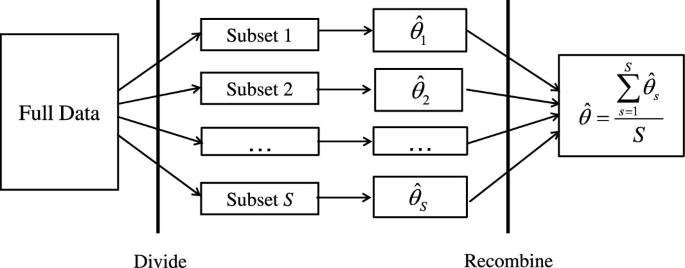
\includegraphics{Divide-recombine.png}
\end{frame}

\hypertarget{non-embarassingly-parallel-problems}{%
\section{Non-embarassingly parallel
problems}\label{non-embarassingly-parallel-problems}}

\begin{frame}{Big Data}
\protect\hypertarget{big-data-1}{}
Map Reduce (Dean and Ghemawat 2008)

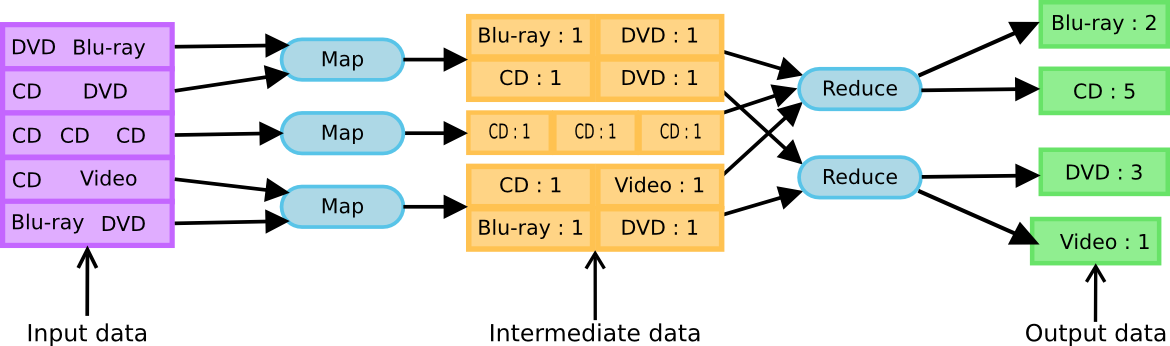
\includegraphics{Map-Reduce.png}
\end{frame}

\hypertarget{examples}{%
\section{Examples}\label{examples}}

\begin{frame}{Natively on RStudio}
\protect\hypertarget{natively-on-rstudio}{}
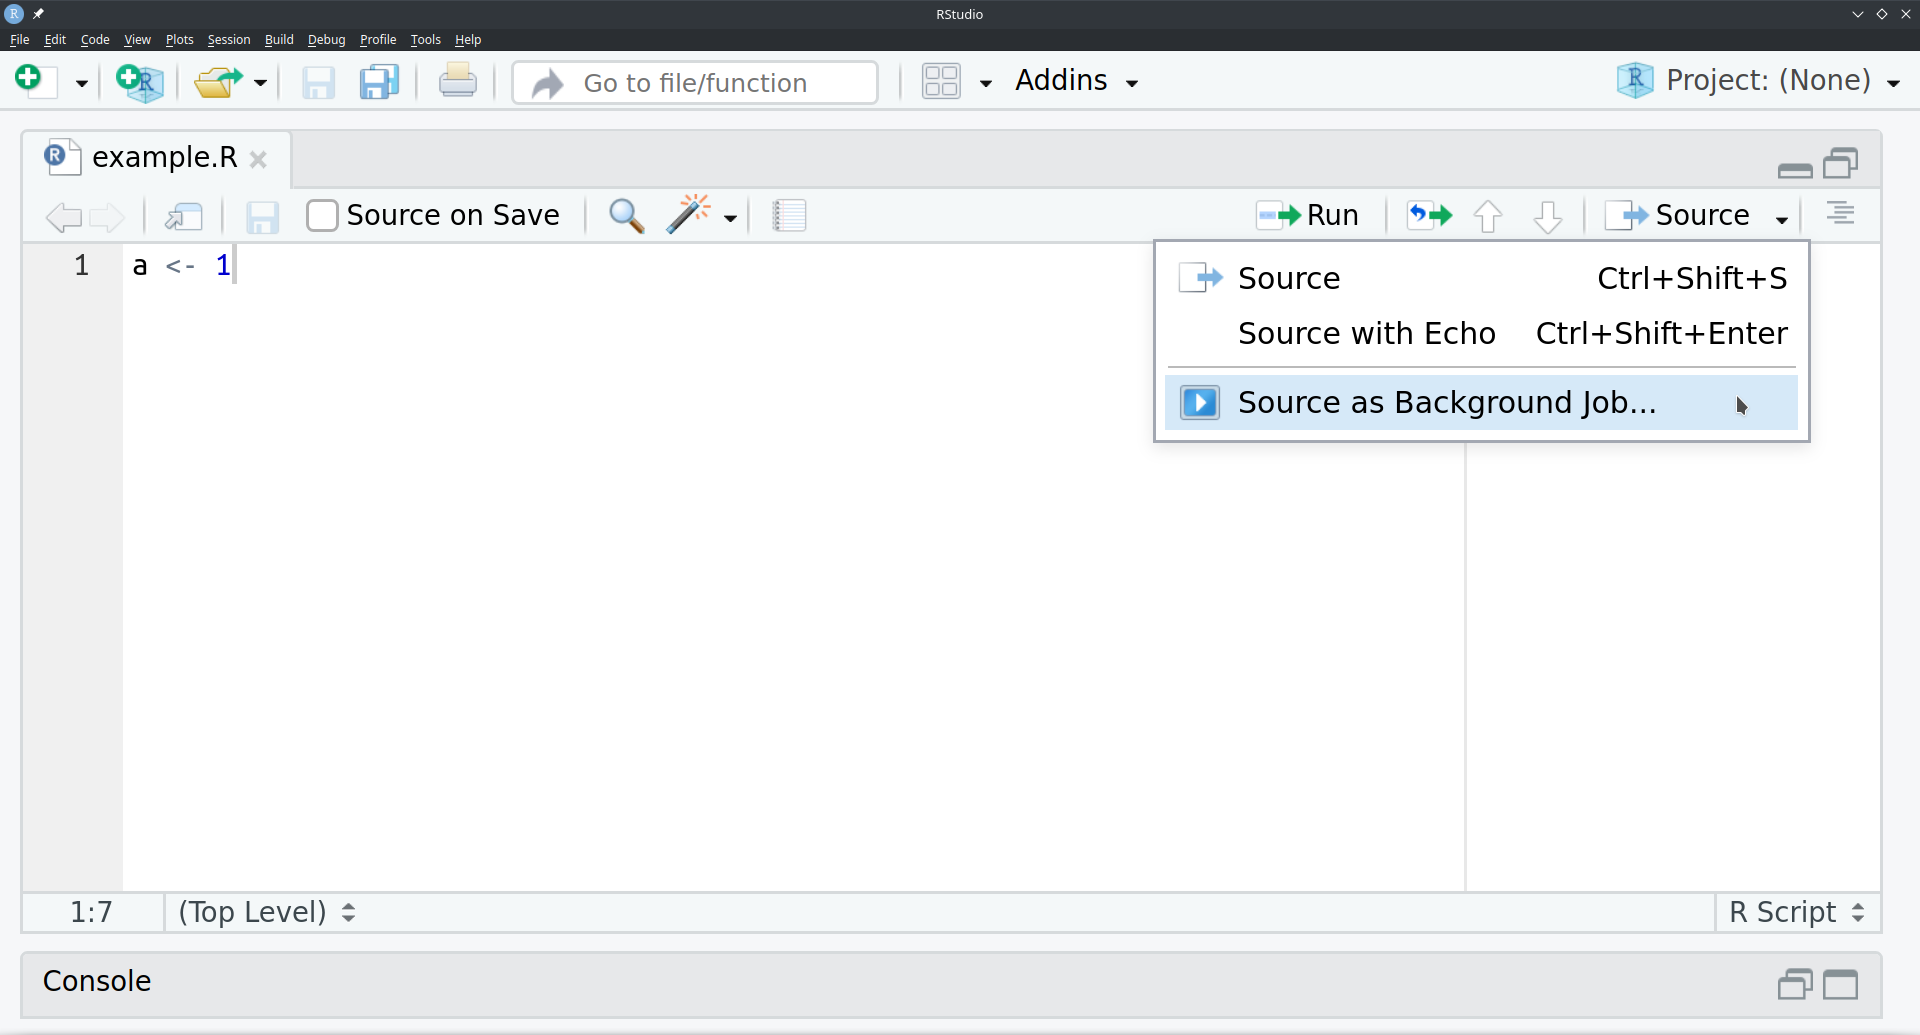
\includegraphics{source background job.png}
\end{frame}

\begin{frame}[fragile]{\texttt{future}}
\protect\hypertarget{future}{}
No worries about

\begin{itemize}
\tightlist
\item
  exporting variables (\texttt{clusterExport})
\item
  packages (\texttt{clusterEvalQ})
\item
  which \texttt{apply} function to use (\texttt{parLapply},
  \texttt{mclapply})
\item
  which parallel back-end to use (\texttt{snow}, \texttt{multicore},
  etc)
\item
  which operating system (Windows, macOS, Linux)
\end{itemize}
\end{frame}

\begin{frame}[fragile]{\texttt{future} basics (1)}
\protect\hypertarget{future-basics-1}{}
\tiny

\begin{Shaded}
\begin{Highlighting}[]
\NormalTok{a }\OtherTok{\textless{}{-}} \FunctionTok{sum}\NormalTok{(}\DecValTok{1}\SpecialCharTok{:}\DecValTok{100}\NormalTok{) }\CommentTok{\# Sequential}
\NormalTok{a}
\end{Highlighting}
\end{Shaded}

\begin{verbatim}
## [1] 5050
\end{verbatim}

\begin{Shaded}
\begin{Highlighting}[]
\FunctionTok{library}\NormalTok{(future)}
\FunctionTok{plan}\NormalTok{(multisession)}
\CommentTok{\# Method 1}
\NormalTok{fb }\OtherTok{\textless{}{-}} \FunctionTok{future}\NormalTok{(\{ }\FunctionTok{sum}\NormalTok{(}\DecValTok{1}\SpecialCharTok{:}\DecValTok{50}\NormalTok{) \})}
\NormalTok{fc }\OtherTok{\textless{}{-}} \FunctionTok{future}\NormalTok{( }\FunctionTok{sum}\NormalTok{(}\DecValTok{51}\SpecialCharTok{:}\DecValTok{100}\NormalTok{) )}
\NormalTok{aa }\OtherTok{\textless{}{-}} \FunctionTok{value}\NormalTok{(fb) }\CommentTok{\# wait until future is resolved}
\NormalTok{aa }\OtherTok{\textless{}{-}}\NormalTok{ aa }\SpecialCharTok{+} \FunctionTok{value}\NormalTok{(fc)}
\NormalTok{aa}
\end{Highlighting}
\end{Shaded}

\begin{verbatim}
## [1] 5050
\end{verbatim}

\begin{Shaded}
\begin{Highlighting}[]
\CommentTok{\# Method 2}
\NormalTok{fb }\SpecialCharTok{\%\textless{}{-}\%}\NormalTok{ \{ }\FunctionTok{sum}\NormalTok{(}\DecValTok{1}\SpecialCharTok{:}\DecValTok{50}\NormalTok{) \}}
\NormalTok{fc }\SpecialCharTok{\%\textless{}{-}\%} \FunctionTok{sum}\NormalTok{(}\DecValTok{51}\SpecialCharTok{:}\DecValTok{100}\NormalTok{)}
\CommentTok{\# fc \%\textless{}{-}\% 1 + 1}
\NormalTok{aaa }\OtherTok{\textless{}{-}}\NormalTok{ fb }\SpecialCharTok{+}\NormalTok{ fc}
\NormalTok{aaa}
\end{Highlighting}
\end{Shaded}

\begin{verbatim}
## [1] 5050
\end{verbatim}

\normalsize
\end{frame}

\begin{frame}[fragile]{\texttt{future} basics (2)}
\protect\hypertarget{future-basics-2}{}
\texttt{apply} and \texttt{map} functions \tiny

\begin{Shaded}
\begin{Highlighting}[]
\FunctionTok{library}\NormalTok{(future.apply)}
\FunctionTok{plan}\NormalTok{(multisession)}
\NormalTok{a }\OtherTok{\textless{}{-}} \FunctionTok{future\_lapply}\NormalTok{(}\DecValTok{1}\SpecialCharTok{:}\DecValTok{5}\NormalTok{, sum)}
\FunctionTok{identical}\NormalTok{(a,}
          \FunctionTok{lapply}\NormalTok{(}\DecValTok{1}\SpecialCharTok{:}\DecValTok{5}\NormalTok{, sum))}
\end{Highlighting}
\end{Shaded}

\begin{verbatim}
## [1] TRUE
\end{verbatim}

\begin{Shaded}
\begin{Highlighting}[]
\CommentTok{\# future\_replicate()}
\CommentTok{\# future\_sapply()}
\CommentTok{\# future\_apply()}

\FunctionTok{library}\NormalTok{(furrr) }\CommentTok{\# futurized \textasciigrave{}purrr\textasciigrave{} package}
\CommentTok{\# future\_map()}
\CommentTok{\# future\_map2()}
\CommentTok{\# future\_modify()}
\end{Highlighting}
\end{Shaded}

\normalsize
\end{frame}

\begin{frame}[fragile]{\texttt{future} Nested loops}
\protect\hypertarget{future-nested-loops}{}
\tiny

\begin{Shaded}
\begin{Highlighting}[]
\FunctionTok{library}\NormalTok{(future)}
\FunctionTok{library}\NormalTok{(listenv)}
\NormalTok{x }\OtherTok{\textless{}{-}} \FunctionTok{listenv}\NormalTok{()}
\FunctionTok{plan}\NormalTok{(}\FunctionTok{list}\NormalTok{(multisession, sequential))}
\ControlFlowTok{for}\NormalTok{ (i }\ControlFlowTok{in} \DecValTok{1}\SpecialCharTok{:}\DecValTok{3}\NormalTok{) \{}
\NormalTok{  x[[i]] }\SpecialCharTok{\%\textless{}{-}\%}\NormalTok{ \{}
    
\NormalTok{    y }\OtherTok{\textless{}{-}} \FunctionTok{listenv}\NormalTok{()}
    \ControlFlowTok{for}\NormalTok{ (j }\ControlFlowTok{in} \DecValTok{1}\SpecialCharTok{:}\DecValTok{3}\NormalTok{) \{}
\NormalTok{      y[[j]] }\SpecialCharTok{\%\textless{}{-}\%}\NormalTok{ \{}
        \FunctionTok{return}\NormalTok{(}\FunctionTok{c}\NormalTok{(}\FunctionTok{Sys.getpid}\NormalTok{(), }\DecValTok{10}\SpecialCharTok{*}\NormalTok{i }\SpecialCharTok{+}\NormalTok{ j))}
\NormalTok{      \}}
\NormalTok{    \}}
    \FunctionTok{return}\NormalTok{(y)}
    
\NormalTok{  \}}
\NormalTok{\}}
\FunctionTok{unlist}\NormalTok{(x)}
\end{Highlighting}
\end{Shaded}

\begin{verbatim}
##  [1] 22664    11 22664    12 22664    13 15980    21 15980    22 15980    23
## [13] 17516    31 17516    32 17516    33
\end{verbatim}

\normalsize
\end{frame}

\begin{frame}[fragile]{\texttt{foreach}}
\protect\hypertarget{foreach}{}
Works with/out any parallel computation back-end

\begin{Shaded}
\begin{Highlighting}[]
\FunctionTok{library}\NormalTok{(foreach)}
\NormalTok{pids }\OtherTok{\textless{}{-}} \FunctionTok{foreach}\NormalTok{(}\AttributeTok{i =} \DecValTok{1}\SpecialCharTok{:}\DecValTok{2}\NormalTok{, }\AttributeTok{.combine =} \StringTok{"c"}\NormalTok{) }\SpecialCharTok{\%do\%}\NormalTok{ \{}
  \FunctionTok{return}\NormalTok{(}\FunctionTok{Sys.getpid}\NormalTok{())}
\NormalTok{\}}
\NormalTok{pids}
\end{Highlighting}
\end{Shaded}

\begin{verbatim}
## [1] 16876 16876
\end{verbatim}
\end{frame}

\begin{frame}[fragile]{\texttt{foreach} (2)}
\protect\hypertarget{foreach-2}{}
\begin{Shaded}
\begin{Highlighting}[]
\FunctionTok{library}\NormalTok{(doFuture)}
\FunctionTok{registerDoFuture}\NormalTok{()}
\FunctionTok{plan}\NormalTok{(}\FunctionTok{multisession}\NormalTok{(}\AttributeTok{workers =} \DecValTok{2}\NormalTok{))}
\NormalTok{pids }\OtherTok{\textless{}{-}} \FunctionTok{foreach}\NormalTok{(}\AttributeTok{i =} \DecValTok{1}\SpecialCharTok{:}\DecValTok{2}\NormalTok{, }\AttributeTok{.combine =} \StringTok{"c"}\NormalTok{) }\SpecialCharTok{\%dopar\%}\NormalTok{ \{}
  \FunctionTok{return}\NormalTok{(}\FunctionTok{Sys.getpid}\NormalTok{())}
\NormalTok{\}}
\NormalTok{pids}
\end{Highlighting}
\end{Shaded}

\begin{verbatim}
## [1] 20612  3184
\end{verbatim}
\end{frame}

\begin{frame}[fragile]{\texttt{foreach} Nested loops}
\protect\hypertarget{foreach-nested-loops}{}
Usually, parallelize the outer loop. \small

\begin{Shaded}
\begin{Highlighting}[]
\FunctionTok{registerDoFuture}\NormalTok{()}
\FunctionTok{plan}\NormalTok{(}\FunctionTok{list}\NormalTok{(}\FunctionTok{tweak}\NormalTok{(multisession, }\AttributeTok{workers =} \DecValTok{3}\NormalTok{),}
          \FunctionTok{tweak}\NormalTok{(multisession, }\AttributeTok{workers =} \DecValTok{2}\NormalTok{)))}
\NormalTok{a }\OtherTok{\textless{}{-}} \FunctionTok{foreach}\NormalTok{(}\AttributeTok{i =} \DecValTok{1}\SpecialCharTok{:}\DecValTok{5}\NormalTok{) }\SpecialCharTok{\%dopar\%}\NormalTok{ \{}
\NormalTok{  a }\OtherTok{\textless{}{-}} \FunctionTok{foreach}\NormalTok{(}\AttributeTok{j =} \DecValTok{1}\SpecialCharTok{:}\DecValTok{5}\NormalTok{) }\SpecialCharTok{\%dopar\%}\NormalTok{ \{}
    \FunctionTok{return}\NormalTok{(}\DecValTok{0}\NormalTok{)}
\NormalTok{  \}}
  \FunctionTok{return}\NormalTok{(}\DecValTok{0}\NormalTok{)}
\NormalTok{\}}
\FunctionTok{plan}\NormalTok{(}\FunctionTok{multisession}\NormalTok{(}\AttributeTok{workers =} \DecValTok{2}\NormalTok{))}
\NormalTok{a }\OtherTok{\textless{}{-}} \FunctionTok{foreach}\NormalTok{(}\AttributeTok{i =} \DecValTok{1}\SpecialCharTok{:}\DecValTok{5}\NormalTok{) }\SpecialCharTok{\%:\%}\NormalTok{ \{}
\NormalTok{  a }\OtherTok{\textless{}{-}} \FunctionTok{foreach}\NormalTok{(}\AttributeTok{j =} \DecValTok{1}\SpecialCharTok{:}\DecValTok{5}\NormalTok{) }\SpecialCharTok{\%dopar\%}\NormalTok{ \{}
    \FunctionTok{return}\NormalTok{(}\DecValTok{0}\NormalTok{)}
\NormalTok{  \}}
  \FunctionTok{return}\NormalTok{(}\DecValTok{0}\NormalTok{)}
\NormalTok{\}}
\end{Highlighting}
\end{Shaded}

\normalsize
\end{frame}

\begin{frame}[fragile]{\texttt{foreach} Chunking tasks}
\protect\hypertarget{foreach-chunking-tasks}{}
Each future will process \texttt{chunk.size} elements (on average).
\small

\begin{Shaded}
\begin{Highlighting}[]
\FunctionTok{registerDoFuture}\NormalTok{()}
\FunctionTok{plan}\NormalTok{(}\FunctionTok{multisession}\NormalTok{(}\AttributeTok{workers =} \DecValTok{2}\NormalTok{))}
\NormalTok{results }\OtherTok{\textless{}{-}} \FunctionTok{foreach}\NormalTok{(}\AttributeTok{i =} \DecValTok{1}\SpecialCharTok{:}\DecValTok{10}\NormalTok{,}
                   \AttributeTok{.options.future =} \FunctionTok{list}\NormalTok{(}\AttributeTok{chunk.size =} \DecValTok{3}\NormalTok{),}
                   \AttributeTok{.combine =} \StringTok{"c"}\NormalTok{) }\SpecialCharTok{\%dopar\%}\NormalTok{ \{}
  \FunctionTok{return}\NormalTok{(}\FunctionTok{Sys.getpid}\NormalTok{())}
\NormalTok{\}}
\NormalTok{results}
\end{Highlighting}
\end{Shaded}

\begin{verbatim}
##  [1] 17820 17820 17820  5800  5800 17820 17820  5800  5800  5800
\end{verbatim}

\normalsize
\end{frame}

\begin{frame}[fragile]{\texttt{foreach} Randomness}
\protect\hypertarget{foreach-randomness}{}
Randomness is a problem.

\begin{Shaded}
\begin{Highlighting}[]
\FunctionTok{set.seed}\NormalTok{(}\DecValTok{1}\NormalTok{)}
\FunctionTok{registerDoFuture}\NormalTok{()}
\FunctionTok{plan}\NormalTok{(}\FunctionTok{multisession}\NormalTok{(}\AttributeTok{workers =} \DecValTok{2}\NormalTok{))}
\NormalTok{results }\OtherTok{\textless{}{-}} \FunctionTok{foreach}\NormalTok{(}\AttributeTok{i =} \DecValTok{1}\SpecialCharTok{:}\DecValTok{2}\NormalTok{, }\AttributeTok{.combine =} \StringTok{"c"}\NormalTok{) }\SpecialCharTok{\%dopar\%}\NormalTok{ \{}
  \FunctionTok{return}\NormalTok{(}\FunctionTok{rnorm}\NormalTok{(}\DecValTok{1}\NormalTok{))}
\NormalTok{\}}
\NormalTok{results}
\end{Highlighting}
\end{Shaded}

\begin{verbatim}
## [1]  1.2335855 -0.2061181
\end{verbatim}

\begin{Shaded}
\begin{Highlighting}[]
\FunctionTok{set.seed}\NormalTok{(}\DecValTok{1}\NormalTok{)}
\FunctionTok{rnorm}\NormalTok{(}\DecValTok{1}\NormalTok{)}
\end{Highlighting}
\end{Shaded}

\begin{verbatim}
## [1] -0.6264538
\end{verbatim}
\end{frame}

\begin{frame}[fragile]{\texttt{foreach} Randomness solution}
\protect\hypertarget{foreach-randomness-solution}{}
\small

\begin{Shaded}
\begin{Highlighting}[]
\FunctionTok{library}\NormalTok{(doRNG)}
\FunctionTok{registerDoFuture}\NormalTok{()}
\FunctionTok{plan}\NormalTok{(multisession, }\AttributeTok{workers =} \DecValTok{2}\NormalTok{)}
\NormalTok{results }\OtherTok{\textless{}{-}} \FunctionTok{foreach}\NormalTok{(}\AttributeTok{i =} \DecValTok{1}\SpecialCharTok{:}\DecValTok{2}\NormalTok{, }\AttributeTok{.combine =} \StringTok{"c"}\NormalTok{) }\SpecialCharTok{\%dorng\%}\NormalTok{ \{}
  \FunctionTok{return}\NormalTok{(}\FunctionTok{rnorm}\NormalTok{(}\DecValTok{1}\NormalTok{))}
\NormalTok{\}}
\NormalTok{results[}\DecValTok{2}\NormalTok{]}
\end{Highlighting}
\end{Shaded}

\begin{verbatim}
## [1] -0.1581411
\end{verbatim}

\begin{Shaded}
\begin{Highlighting}[]
\NormalTok{.Random.seed }\OtherTok{\textless{}{-}} \FunctionTok{attr}\NormalTok{(results, }\StringTok{"rng"}\NormalTok{)[[}\DecValTok{2}\NormalTok{]]}
\FunctionTok{rnorm}\NormalTok{(}\DecValTok{1}\NormalTok{)}
\end{Highlighting}
\end{Shaded}

\begin{verbatim}
## [1] -0.1581411
\end{verbatim}

\normalsize
\end{frame}

\begin{frame}[fragile]{Monitoring}
\protect\hypertarget{monitoring}{}
\small

\begin{Shaded}
\begin{Highlighting}[]
\FunctionTok{library}\NormalTok{(mailR)}
\NormalTok{myemail }\OtherTok{\textless{}{-}} \StringTok{"riw011@uib.no"}
\CommentTok{\# Email}
\NormalTok{message }\OtherTok{\textless{}{-}} \StringTok{"May the force be with you"}
\FunctionTok{send.mail}\NormalTok{(}\AttributeTok{from =}\NormalTok{ myemail,}
          \AttributeTok{to =}\NormalTok{ myemail,}
          \AttributeTok{subject =} \StringTok{"Hello there"}\NormalTok{,}
          \AttributeTok{body =}\NormalTok{ message,}
          \AttributeTok{smtp =} \FunctionTok{list}\NormalTok{(}\AttributeTok{host.name =} \StringTok{"smtp.uib.no"}\NormalTok{,}
                      \AttributeTok{user.name =}\NormalTok{ myemail,}
                      \AttributeTok{passwd =}\NormalTok{ mypassword))}
\CommentTok{\# Online service}
\FunctionTok{system}\NormalTok{(}\FunctionTok{paste0}\NormalTok{(}\StringTok{\textquotesingle{}curl {-}d "\textquotesingle{}}\NormalTok{, message,}\StringTok{\textquotesingle{}" ntfy.sh/aaaa\textquotesingle{}}\NormalTok{))}
\end{Highlighting}
\end{Shaded}

\normalsize
\end{frame}

\begin{frame}[fragile]{Monitoring with progress bar}
\protect\hypertarget{monitoring-with-progress-bar}{}
\tiny

\begin{Shaded}
\begin{Highlighting}[]
\FunctionTok{library}\NormalTok{(doFuture)}
\FunctionTok{library}\NormalTok{(progressr)}
\FunctionTok{registerDoFuture}\NormalTok{()}
\FunctionTok{plan}\NormalTok{(}\FunctionTok{multisession}\NormalTok{(}\AttributeTok{workers =} \DecValTok{2}\NormalTok{))}

\CommentTok{\# Monitoring this function}
\NormalTok{aa }\OtherTok{\textless{}{-}} \ControlFlowTok{function}\NormalTok{() \{}
\NormalTok{  p }\OtherTok{\textless{}{-}} \FunctionTok{progressor}\NormalTok{(}\AttributeTok{along =} \DecValTok{1}\SpecialCharTok{:}\DecValTok{10}\NormalTok{)}
  \FunctionTok{foreach}\NormalTok{(}\AttributeTok{i =} \DecValTok{1}\SpecialCharTok{:}\DecValTok{10}\NormalTok{) }\SpecialCharTok{\%dopar\%}\NormalTok{ \{}
    \FunctionTok{Sys.sleep}\NormalTok{(}\DecValTok{2}\NormalTok{)}
    \FunctionTok{p}\NormalTok{() }\CommentTok{\# Increment progress bar}
    \FunctionTok{return}\NormalTok{(}\ConstantTok{NULL}\NormalTok{)}
\NormalTok{  \}}
  \FunctionTok{return}\NormalTok{(}\ConstantTok{NULL}\NormalTok{)}
\NormalTok{\}}

\CommentTok{\# Method 1}
\FunctionTok{handlers}\NormalTok{(}\AttributeTok{global =} \ConstantTok{TRUE}\NormalTok{)}
\FunctionTok{aa}\NormalTok{()}

\CommentTok{\# Method 2}
\FunctionTok{handlers}\NormalTok{(}\AttributeTok{global =} \ConstantTok{FALSE}\NormalTok{)}
\FunctionTok{with\_progress}\NormalTok{(\{}
  \FunctionTok{aa}\NormalTok{()}
\NormalTok{\})}
\end{Highlighting}
\end{Shaded}

\normalsize
\end{frame}

\begin{frame}{Monitoring}
\protect\hypertarget{monitoring-1}{}
\movie[width=10cm,height=6cm]{Laplacian 2D}{monitoring_progress_bar.mp4}
\end{frame}

\begin{frame}[fragile]{Race condition / concurrent writing}
\protect\hypertarget{race-condition-concurrent-writing}{}
\tiny

\begin{Shaded}
\begin{Highlighting}[]
\FunctionTok{library}\NormalTok{(doFuture)}
\FunctionTok{registerDoFuture}\NormalTok{()}
\FunctionTok{plan}\NormalTok{(multisession, }\AttributeTok{workers =} \DecValTok{11}\NormalTok{)}
\NormalTok{a }\OtherTok{\textless{}{-}} \FunctionTok{foreach}\NormalTok{(}\AttributeTok{i =} \DecValTok{1}\SpecialCharTok{:}\DecValTok{1000}\NormalTok{) }\SpecialCharTok{\%dopar\%}\NormalTok{ \{}
  \FunctionTok{write}\NormalTok{(}\StringTok{"Dude"}\NormalTok{, }\AttributeTok{file =} \StringTok{"log.txt"}\NormalTok{, }\AttributeTok{append =} \ConstantTok{TRUE}\NormalTok{)}
  \FunctionTok{write}\NormalTok{(}\StringTok{"where"}\NormalTok{, }\AttributeTok{file =} \StringTok{"log.txt"}\NormalTok{, }\AttributeTok{append =} \ConstantTok{TRUE}\NormalTok{)}
  \FunctionTok{write}\NormalTok{(}\StringTok{"is"}\NormalTok{, }\AttributeTok{file =} \StringTok{"log.txt"}\NormalTok{, }\AttributeTok{append =} \ConstantTok{TRUE}\NormalTok{)}
  \FunctionTok{write}\NormalTok{(}\StringTok{"my"}\NormalTok{, }\AttributeTok{file =} \StringTok{"log.txt"}\NormalTok{, }\AttributeTok{append =} \ConstantTok{TRUE}\NormalTok{)}
  \FunctionTok{write}\NormalTok{(}\StringTok{"car"}\NormalTok{, }\AttributeTok{file =} \StringTok{"log.txt"}\NormalTok{, }\AttributeTok{append =} \ConstantTok{TRUE}\NormalTok{)}
  \FunctionTok{return}\NormalTok{(}\ConstantTok{NA}\NormalTok{)}
\NormalTok{\}}
\NormalTok{fpeek}\SpecialCharTok{::}\FunctionTok{peek\_tail}\NormalTok{(}\StringTok{"log.txt"}\NormalTok{, }\AttributeTok{n =} \DecValTok{50}\NormalTok{, }\AttributeTok{intern =} \ConstantTok{TRUE}\NormalTok{)}
\end{Highlighting}
\end{Shaded}

\begin{verbatim}
##  [1] "r"             ""              "iscar"         "Dude"         
##  [5] "my"            "Dude"          ""              "wherecarhere" 
##  [9] ""              "car"           "isdeis"        "Dude"         
## [13] "ere"           "my"            ""              "is"           
## [17] "ere"           "carcar"        "is"            ""             
## [21] "DudeDude"      ""              "car"           ""             
## [25] "wherewherecar" ""              "Dude"          "is"           
## [29] "iswhere"       "mymy"          "is"            "car"          
## [33] "carmy"         ""              "Dude"          "car"          
## [37] "where"         "Dude"          "is"            "where"        
## [41] "my"            "is"            "car"           "my"           
## [45] "car"           "Dude"          "where"         "is"           
## [49] "my"            "car"
\end{verbatim}

\normalsize
\end{frame}

\begin{frame}[fragile]{Race condition solution}
\protect\hypertarget{race-condition-solution}{}
\texttt{filelock} (does not work well) or \texttt{flock} package

\tiny

\begin{Shaded}
\begin{Highlighting}[]
\FunctionTok{library}\NormalTok{(doFuture)}
\FunctionTok{registerDoFuture}\NormalTok{()}
\FunctionTok{plan}\NormalTok{(multisession, }\AttributeTok{workers =} \DecValTok{11}\NormalTok{)}
\NormalTok{a }\OtherTok{\textless{}{-}} \FunctionTok{foreach}\NormalTok{(}\AttributeTok{i =} \DecValTok{1}\SpecialCharTok{:}\DecValTok{1000}\NormalTok{, }\AttributeTok{.packages =} \StringTok{"flock"}\NormalTok{) }\SpecialCharTok{\%dopar\%}\NormalTok{ \{}
  
\NormalTok{  mylock }\OtherTok{\textless{}{-}} \FunctionTok{lock}\NormalTok{(}\StringTok{"lockfile"}\NormalTok{)}
  \FunctionTok{write}\NormalTok{(}\StringTok{"Hasta"}\NormalTok{, }\AttributeTok{file =} \StringTok{"log2.txt"}\NormalTok{, }\AttributeTok{append =} \ConstantTok{TRUE}\NormalTok{)}
  \FunctionTok{write}\NormalTok{(}\StringTok{"la"}\NormalTok{, }\AttributeTok{file =} \StringTok{"log2.txt"}\NormalTok{, }\AttributeTok{append =} \ConstantTok{TRUE}\NormalTok{)}
  \FunctionTok{write}\NormalTok{(}\StringTok{"vista"}\NormalTok{, }\AttributeTok{file =} \StringTok{"log2.txt"}\NormalTok{, }\AttributeTok{append =} \ConstantTok{TRUE}\NormalTok{)}
  \FunctionTok{write}\NormalTok{(}\StringTok{"baby"}\NormalTok{, }\AttributeTok{file =} \StringTok{"log2.txt"}\NormalTok{, }\AttributeTok{append =} \ConstantTok{TRUE}\NormalTok{)}
  \FunctionTok{unlock}\NormalTok{(mylock)}
  
  \FunctionTok{return}\NormalTok{(}\ConstantTok{NA}\NormalTok{)}
\NormalTok{\}}
\NormalTok{fpeek}\SpecialCharTok{::}\FunctionTok{peek\_tail}\NormalTok{(}\StringTok{"log2.txt"}\NormalTok{, }\AttributeTok{n =} \DecValTok{50}\NormalTok{, }\AttributeTok{intern =} \ConstantTok{TRUE}\NormalTok{)}
\end{Highlighting}
\end{Shaded}

\begin{verbatim}
##  [1] "vista" "baby"  "Hasta" "la"    "vista" "baby"  "Hasta" "la"    "vista"
## [10] "baby"  "Hasta" "la"    "vista" "baby"  "Hasta" "la"    "vista" "baby" 
## [19] "Hasta" "la"    "vista" "baby"  "Hasta" "la"    "vista" "baby"  "Hasta"
## [28] "la"    "vista" "baby"  "Hasta" "la"    "vista" "baby"  "Hasta" "la"   
## [37] "vista" "baby"  "Hasta" "la"    "vista" "baby"  "Hasta" "la"    "vista"
## [46] "baby"  "Hasta" "la"    "vista" "baby"
\end{verbatim}

\normalsize
\end{frame}

\hypertarget{parallel-computing-at-scale}{%
\section{Parallel computing at
scale}\label{parallel-computing-at-scale}}

\begin{frame}[fragile]{Parallel computing at scale}
\footnotesize

\begin{block}{Distributed computing}
\protect\hypertarget{distributed-computing}{}
\begin{itemize}
\tightlist
\item
  \href{mailto:Seti@Home}{\nolinkurl{Seti@Home}} with BOINC software
\item
  \href{mailto:Folding@Home}{\nolinkurl{Folding@Home}}, about protein
  folding
\item
  Fold.it puzzle video game
\end{itemize}
\end{block}

\begin{block}{Apache Hadoop}
\protect\hypertarget{apache-hadoop}{}
Google's Map-Reduce
\end{block}

\begin{block}{Apache Spark}
\protect\hypertarget{apache-spark}{}
More efficient on smaller but still massive data sets
\end{block}

\begin{block}{More efficient tools}
\protect\hypertarget{more-efficient-tools}{}
\begin{itemize}
\tightlist
\item
  Schedulers: SLURM
\item
  MPI (Message Programming Interface) with package \texttt{rmpi} is
  de-facto standard
\item
  Managing shared memory processes with e.g.~POSIX Threads or OpenMP
\end{itemize}

e.g. (de Vicente and Rodriguez 2005) uses specialized tools to manage a
dynamic cluster of non-dedicated workstations \normalsize
\end{block}
\end{frame}

\hypertarget{references}{%
\section{References}\label{references}}

\begin{frame}{References}
\hypertarget{refs}{}
\begin{CSLReferences}{1}{0}
\leavevmode\vadjust pre{\hypertarget{ref-dean}{}}%
Dean, Jeffrey, and Sanjay Ghemawat. 2008. {``{MapReduce}: Simplified
Data Processing on Large Clusters.''} \emph{Communications of the ACM}
51 (1): 107--13. \url{https://doi.org/10.1145/1327452.1327492}.

\leavevmode\vadjust pre{\hypertarget{ref-guha}{}}%
Guha, Saptarshi, Ryan Hafen, Jeremiah Rounds, Jin Xia, Jianfu Li, Bowei
Xi, and William S. Cleveland. 2012. {``Large Complex Data: Divide and
Recombine ({D}\&{R}) with {RHIPE}.''} \emph{Stat} 1 (1): 53--67.
\url{https://doi.org/10.1002/sta4.7}.

\leavevmode\vadjust pre{\hypertarget{ref-devicente}{}}%
Vicente, Angel de, and Nayra Rodriguez. 2005. {``Big Science with a
Small Budget: {Non-embarrassingly} Parallel Applications in a
Non-Dedicated Network of Workstations.''} {arXiv}.
\url{https://doi.org/10.48550/ARXIV.CS/0510094}.

\end{CSLReferences}
\end{frame}

\end{document}
